The development process during the project has been extremely agile. We took full advantage of the fact that we sit all developers together every day and have near perfect and instant information sharing\todokasper{This sentence seems a tad dangerous, perhaps we should leave it out.}. The general idea was to come up with major features, each of which were decomposed to an issue, an example of this can be seen in \ref{evaluation:workprocess:issue}. 

\begin{figure}[H]
\centering
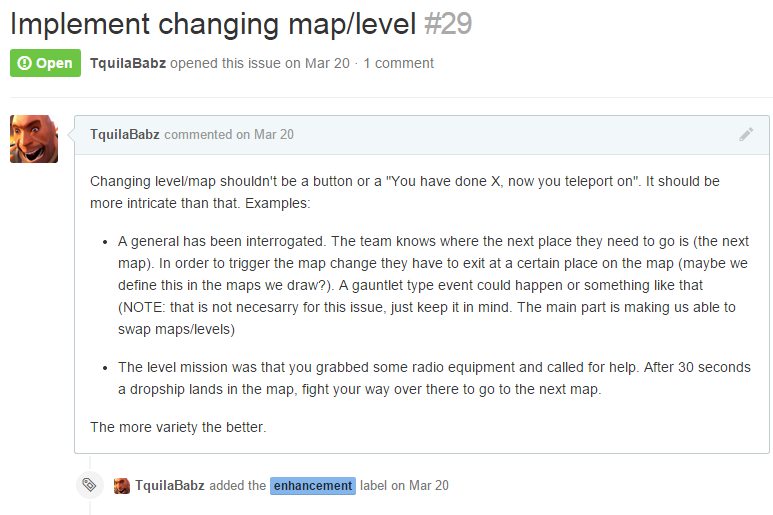
\includegraphics[width=1\textwidth]{figures/evaluation/issue}
\caption{Example of an actual issue on our issue tracker.}
\label{evaluation:workprocess:issue}
\end{figure}

Further, these issues were attached to very rough milestones describing what was intended for the milestone, a rough milestone can be seen in \ref{evaluation:workprocess:milestone}

\begin{figure}[H]
\centering
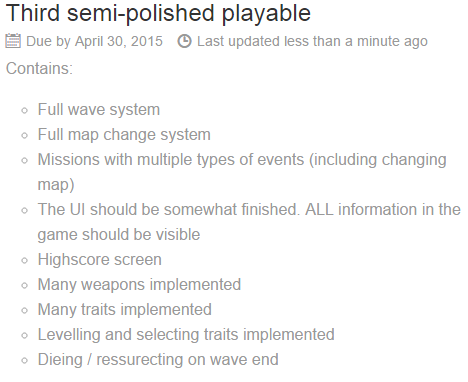
\includegraphics[width=1\textwidth]{figures/evaluation/milestone}
\caption{Part of a milestone with rough description of required elements}
\label{evaluation:workprocess:milestone}
\end{figure}

Each issue would be rather loosely defined in terms of the precise architecture needed to be implemented in order to facilitate the issue, and generally this task was handled by the person/persons who were attached to the issue. 

A lot of issue prioritization was done on the fly, and this responsibility would generally be entrusted to the people dealing with the area of concern. If anything needed more elaboration the team members would simply ask for an ensemble and the issue of concern would be discussed through in more detail in the entire group. The amount of people involved with the current issue would then come up with a direction for which the development would go, and the entire team would be updated on the new state of the development process. In essence, the competences of the group was high enough that in most cases, we did not need to elaborate further on architectural choices, and the team members had the insight needed to know when to ask questions regarding architectural design which had an influence on what they were developing. 
It is obvious this only works because we know the project extremely well, and have a relatively small team. Further there was no need to information share to people who are not \emph{in the middle of it all}.